\section{Design}
\label{sec:design}

In order to better utilize the various servers in a distributed database and prevent servers from becoming hotspots, we have designed a method to assign jobs based on server conditions. A program runs on all of the servers in the cluster and periodically measures the servers' resource usage (e.g., CPU Usage). When the master server receives a query from a client it examines the resource usage of all the servers in the cluster. It chooses the server with the lowest resource usage (the one that is the most likely to finish a query fastest) to assign the query to. In this way, we will hopefully mitigate hotspots on node servers, balance the workload and eventually improve the overall performance of the database. In the remainder of this section, we will state our assumptions about the working environment, give a detailed description of the overall design and provide a typical example of how the program will flow.

\subsection{Assumptions}
For scoping reasons we have made several assumptions about the database:

\begin{itemize}

\item The ultimate goal for this project is to make a methodology that is generally applicable to any kind of database. However, in this project, we will only focus on distributed key-value databases.

\item We only consider database setups that have a  that have a single master server. This is done to reduce the complexity of the clusters that we consider in our design. Because a single master server handles the whole system, we focused on reducing the overhead of the master server (which will be discussed in more detail in Section~\ref{sec:implementation}).

\end{itemize}

We have created two different programs that will measure the resource usage of each node and collect the resource usage information of each node on the master server.

The program running on every node is called the Resource Monitor(RM). The RM measures the server conditions by measuring values such as the CPU and Memory (RAM) usage. After obtaining the resource usage values, a resource usage score is calculated using the following equation:

\begin{center}
$ResourceUsage = \frac{1}{1-CPU} \times \frac{1}{1-Memory}$
\end{center}

The $CPU$ value is the CPU usage of the machine as a percentage value between 0 and 1. The $Memory$ value is a ratio of the used memory divided by the total memory. The formula above has been shown in previous work to be a good indicator of the computing cability of a server~\cite{Wood:2007:BGS:1973430.1973447}.

The program running on the master server is called the Central Job Director (CJD). The CJD is responsible for collecting the resource usage scores from the RMs and determining which node should be assigned a particular query.

Figure~\ref{fig:designFig} illustrates how the communication between the RM, CJD and database occurs. The resource usage score is periodically sent from the RM to the CJD. By passively receiving the resource scores the master server can get the updated node server condition with very little overhead. If the master server were to ask for the score actively there would not only be twice as many network messages to retrieve the resource score, but there would also be the possibility of the CJD becoming blocked and waiting for a reply from a node server. The only downside of doing it this way is that the RM must be aware of the IP address of the master server. After collecting the scores, the CJD stores them and makes them available through an API to the database. The database can use these values to determine the optimal location to process a query. The exact method of communication between the CJD and database will be discussed in more detail in Section~\ref{sec:implementation}.

\begin{figure}[t]
\centering
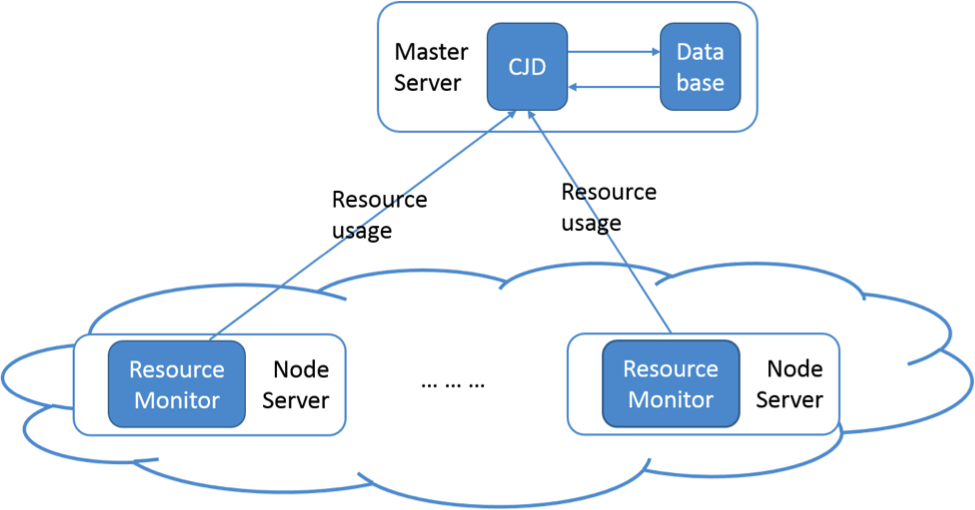
\includegraphics[scale=0.5]{images/design.png}
\caption{The physical design of a cluster using our resource usage based query assignment algorithm.}
\label{fig:designFig}
\end{figure}

\section{Implementation}
\label{sec:implementation}
In this section, we present the detailed implementation methodology for our scheduling algorithm. In the implementation used in our project we are using Apache Cassandra~\cite{ Lakshman:2010:CDS:1773912.1773922}. To scope our project, we only implemented the algorithm for single-key reads and scans. In the remainder of this section we will first present the implementations of the RM, CJD, and the modifications to Cassandra.

\subsection{The Resource Monitor}
The RM resides on each of the node servers in the cluster. To measure the CPU and Memory usage of the server we are using JavaSysMon\footnote{https://github.com/jezhumble/javasysmon}. Every 1 second the RM sends a UDP packet containing its resource usage score to the CJD server. We chose a 1 second interval because we do not feel that the increased information gained by a smaller interval is enough to justify the increased overhead on the network and server processing ability. In addition, given the relatively short amount of time it takes to process a query (even scans) we do not believe it is possible for the RM to send packets fast enough that the algorithm can its assignment decision based on the execution of a single query. For these reasons we are more interested in determining if a node is being consistently heavily loaded, so that we can assign queries to other nodes in the cluster.

\subsection{The Central Job Director}
The CJD runs as a separate program on the master server and is responsible for collecting resource scores of all node servers, storing the data and making that data available to the database. It listens to the network and receives all of the UDP packets from the RMs. Each packet provides the node address and resource usage value for that node. This information is then stored in a hash table. To make the resource usage information available to the database we are using Java’s Remote Method Invocation~\cite{JavaRMI}. The database can then call the remote method (this is straightforward with Cassandra as it is written in Java) and retrieve the hash table containing the node addresses and their resource usages.

\subsection{Cassandra}
We have chosen to diverge from our original design and implement the assignment logic within Cassandra instead of the CJD (to reduce the number of inter-process calls). We modified the Cassandra code that performs single-key reads to assign a query to the replica that has the lowest resource usage. The exception to this is the case where a replica is already located on the master server, at which point we always assign the query to the master (to avoid needing the additional network communication). This part of code is extremely critical because it runs every time the database receives a read query. If it is slow, the performance of the database will be bad no matter how accurate the resource usage score is. We will discuss how we reduced the overhead in Section~\ref{sec:impl_overhead}.

The assignment logic for scans is similar to the logic for reads, but it also considers that the range of keys may exist on several different replicas.

We should note that the CJD could have been implemented within Cassandra (as they both exist on the same server). However, we chose to keep them separate to reduce the coupling of our method to Cassandra and make things easier to move around on the cluster.

\subsection{Reducing overhead}
\label{sec:impl_overhead}
